%\documentclass[10pt]{article}
\documentclass{amsart}
\usepackage{amsmath}
\usepackage{amsthm}
\usepackage{amssymb}
\usepackage{mathrsfs}
\usepackage{hyperref}
%\usepackage{chngcntr}
\usepackage[left=2.5cm,top=2cm,right=2.5cm,bottom=2cm,head=.95cm,foot=.95cm]{geometry}
%\usepackage{bbding}
\usepackage{pifont}
\usepackage{tikz}
\usetikzlibrary{matrix,arrows}
%\usepackage{listofitems}
%\usepackage{stackengine}
%\stackMath
%\setstackgap{S}{1pt}
\usepackage{wasysym}
\usepackage{graphicx}
\usepackage{wrapfig}
\usepackage{subcaption}
\usepackage{mwe}
\usepackage{float}
%\usepackage[htt]{hyphenat}


%\counterwithin{equation}{section}




\makeatletter
\newtheorem*{rep@theorem}{\rep@title}
\newcommand{\newreptheorem}[2]{%
\newenvironment{rep#1}[1]{%
 \def\rep@title{#2 \ref{##1}}%
 \begin{rep@theorem}}%
 {\end{rep@theorem}}}
\makeatother


\newtheorem{thm}{Theorem}[section]
\newreptheorem{thm}{Theorem}
\newtheorem{prop}[thm]{Proposition} 
\newreptheorem{prop}{Proposition}
\newtheorem{conj}[thm]{Conjecture}
\newtheorem{lem}[thm]{Lemma}
\newreptheorem{lem}{Lemma}
\newtheorem{cor}[thm]{Corollary}
\newtheorem*{blankthm}{Theorem}
\newtheorem*{blankcor}{Corollary}



\theoremstyle{definition}
\newtheorem{dfn}[thm]{Definition}
\newtheorem{exmpl}[thm]{Example}
\newtheorem{?}[thm]{Question}
\newtheorem*{blankdfn}{Definition}
\newtheorem*{probstat}{Problem Statement}

\theoremstyle{remark}
\newtheorem{rmk}[thm]{Remark}

\newcommand{\HOM}{\mathbb{H}\text{om}}
\newcommand{\FR}{\mathfrak}
\newcommand{\ds}{\displaystyle}
\newcommand{\tql}{\textquotedblleft}
\newcommand{\tqr}{\textquotedblright}
\newcommand{\noin}{\noindent}
\newcommand{\mc}{\mathcal}
\newcommand{\mb}{\mathbb}
\newcommand{\mbf}{\mathbf}
\newcommand{\openstar}{\text{\ding{73}}}
\newcommand{\peq}{\preceq}
\newcommand{\seq}{\succeq}
%\newcommand{\nci}{\Shortstack{. . . .}} 
\newcommand{\nci}{\large{\vdots}}
\newcommand{\bb}{$\bullet\bullet$}
\newcommand{\bbb}{$\bullet\bullet\bullet$}


%\begin{figure}[!htb]
%\centering
%\includegraphics[width=12cm]{num_students_in_20_years.jpeg}
%\captionof{figure}{\small{Histogram of the number of students produced in the first 20 years of a career on a logscale}}
%\label{fig:num_students_in_20_years} 
%\end{figure}


\begin{document}
   \def\lfhook#1{\setbox0=\hbox{#1}{\ooalign{\hidewidth
    \lower1.5ex\hbox{'}\hidewidth\crcr\unhbox0}}} 
\title{Is your advice unethical?}
\author{Scott Atkinson}


\maketitle

\section{Introduction}

Ethics is an important facet of civilization, and a community's ability to discern between ethical and unethical behavior is critical for a healthy society.  In any business, school, or community, ethical communication and behavior is of high importance. For many situations, it is not difficult to decide if an action is ethical or not, but there are also many scenarios lying in an ethical gray area.  The growing scale of text communication makes moderating social media sites, internal business communication platforms, and other online forums impossible to do manually--calling for an automated approach to detect unethical behavior. 

This project applies machine learning techniques to try to statistically detect ethical advice and answer the question: \textbf{What makes a piece of advice unethical?}  
We will use data from two subreddits on the Reddit website: LifeProTips and UnethicalLifeProTips.  For most of the posts in these subreddits, a typical well-adjusted adult will be able to accurately classify them into their proper subreddits. That is, there are not that many \tql ethically gray\tqr posts in our dataset.  So it is a reasonable expectation that a binary classification model can be trained to flag unethical advice. 

Our analysis shows some general trends in the nature of the posts coming from the two subreddits. Advice coming from LifeProTips is generally aimed toward self-improvement.  That is, most of the tips involve actions an individual can take to improve the quality of their life. These actions typically do not depend on the cooperation or participation of any other individual.  For example:
\begin{itemize}
\item \begin{quote}
\tql hold both ends of the tube and run it over the edge of the sink to push toothpaste to the top - you'll get almost every last bit with almost no effort\tqr
\end{quote}
\end{itemize}
On the other hand, the pieces of advice coming from UnethicalLifeProTips generally involve some sort of dishonest behavior an individual can adopt with the goal of gaining some sort of advantage (financial, social, emotional, or otherwise) from someone else, often at their (the other's) expense.  For example:
\begin{itemize}
\item \begin{quote}
\tql The best way to hang up on someone is in the middle of your own sentence. That way they never suspect you of hanging up on them.\tqr
\end{quote}
\end{itemize}
So the labels for this binary classification problem can be set to \tql self-improvement\tqr or \tql dishonesty with the purpose of gaining from others.\tqr When one really thinks about it, one could conclude that the purpose of all dishonesty is to gain from someone else.

In \S \ref{data}, we discuss the data sources, data preparation, and data analysis.  In particular, we examine some expected word frequencies, compare reading levels across the subreddits, and cluster the posts to find some common topics. We also assess the most predictive words for each label with a multinomial naive Bayes analysis.  In \S\ref{modeling} we assess and select our classification model and the proper threshold for the intended use of our model.  In \S\ref{conclusion} we draw our conclusions on our findings and discuss potential improvements for the model.



%\begin{probstat}
%
%\end{probstat}


\section{Data}\label{data}

\subsection{Data sources}

The data for this project are obtained from two subreddits on the online forum site \href{https://www.reddit.com/}{www.reddit.com}: \href{https://www.reddit.com/r/LifeProTips/}{LifeProTips}  and \href{https://www.reddit.com/r/UnethicalLifeProTips/}{UnethicalLifeProTips}.  The LifeProTips subreddit contains user-generated content in the form of advice, hints, and tips for various things.  The UnethicalLifeProTips subreddit contains similar content with the difference being that the tips are unethical, or at best, in an ethical gray area.  The data was obtained by scraping the most recent 5000 posts from each subreddit in early January 2021 using the \texttt{pushshift} API. The posts collected run the spectrum from making you laugh to making you cringe. 
%To warm up we record two posts from each subreddit. 
%
%\noin From LifeProTips:
%
%\begin{itemize}
%
%\item \begin{quote}
%\tql hold both ends of the tube and run it over the edge of the sink to push toothpaste to the top - you'll get almost every last bit with almost no effort\tqr
%\end{quote}
%
%\item \begin{quote}
%\tql Always download and read the User Manual before buying expensive appliances and electronics, you will often find details not mentioned in the marketing material that will influence your buying decision\tqr
%\end{quote}
%
%\end{itemize}
%
%\noin From UnethicalLifeProTips:
%
%\begin{itemize}
%
%\item \begin{quote}
%\tql The best way to hang up on someone is in the middle of your own sentence. That way they never suspect you of hanging up on them.\tqr
%\end{quote}
%
%\item \begin{quote}
%\tql Add \tql21\tqr to the end of handwritten dates in a MM-DD-YY format that expire in 2020.\tqr
%\end{quote}
%
%\end{itemize}
%
We will see samples from each subreddit throughout the report.

\subsection{Data preparation and analysis}

The data from each subreddit were assembled into their own respective dataframes with the following attributes: \texttt{subreddit, title, id, created\_utc, score, num\_comments, selftext}.  For training purposes, we concatenate the two dataframes into a single dataframe.  The \texttt{subreddit} column serves as our label/target column. In the \texttt{title} and \texttt{selftext} columns, we pass all letters to lowercase and remove all punctuation.  We also remove all instances of the abbreviations \tql lpt\tqr and \tql ulpt\tqr along with any appearance of \tql unethical.\tqr After cleaning, LifeProTips has 4945 entries, and UnethicalLifeProTips has 4926 entries in the dataset.

After a preliminary look at some entries for each subreddit, we form a list of some words that could be predictive for each and compare their frequencies for each subreddit.  Figure \ref{fig:word_freq_diff} provides a visualization for some of the differences between the word frequencies.  From a preliminary check of the two subreddits, LifeProTips appears has many pieces of advice telling you not to do one thing and to do another thing instead, and UnethicalLifeProTips evidently has many posts about how to pay less or no money for goods or services.

\begin{figure}
\centering
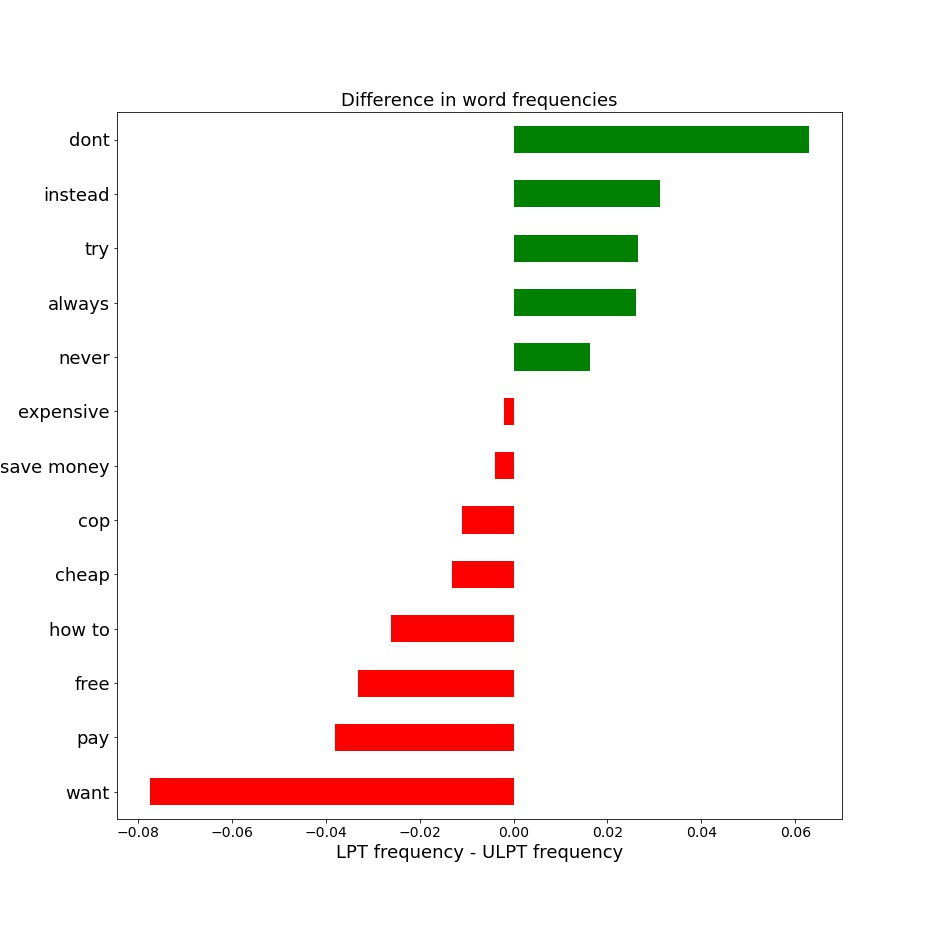
\includegraphics[width=12cm]{prelim_word_freq.jpeg}
\captionof{figure}{\small{Difference in frequencies of words in each subreddit}}
\label{fig:word_freq_diff} 
\end{figure}

We next consider the reading levels of the posts from each subreddit.  We used the \texttt{flesch\_kincaid\_grade} reading level function from the \texttt{textstat} module to evaluate the reading levels of the \emph{unprocessed} title post.  The Flesch-Kincaid grade level is given by the following formula. \[0.39\left(\frac{\text{total words}}{\text{total sentences}} \right) + 11.8\left(\frac{\text{total syllables}}{\text{total words}}\right) - 15.59\]  The output returned is meant to roughly align with U.S. grade levels.  We retain the punctuation for the reading level computation because sentence count needs to be taken into account. We pass this value to the \texttt{title\_reading\_level} column of the dataframe. The summary data returned is included in Table \ref{readinglevels}, and Figure \ref{readinglevel_boxplot} displays the box plots for reading level of \texttt{title} by subreddit.

\begin{figure}
\centering
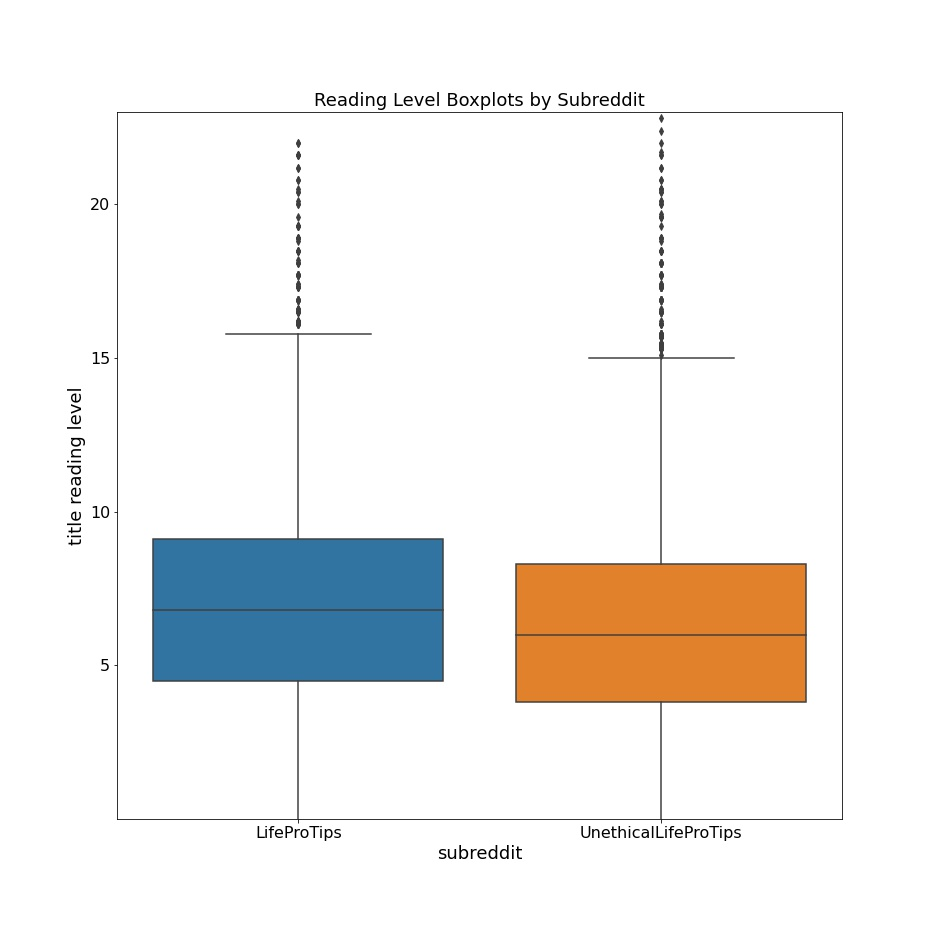
\includegraphics[width=12cm]{readinglevel_boxplot.jpeg}
\captionof{figure}{\small{Box plots displaying the distribution of reading levels for the titles grouped by subreddit}}
\label{readinglevel_boxplot} 
\end{figure}

\begin{table}
\caption{Flesch-Kincaid grade levels for \texttt{title}}\label{readinglevels}
\begin{tabular}{|p{0.2\linewidth}|p{0.1\linewidth}|p{0.1\linewidth}|p{0.1\linewidth}|p{0.1\linewidth}|p{0.13\linewidth}|}
\hline
subreddit & mean & std & Q1 & median & Q3\\
\hline
LifeProTips & 7.0028 & 3.5783 & 4.5   & 6.8 & 9.1 \\
\hline
UnethicalLifeProTips & 6.3536 & 3.8397 &  3.8  & 6.0 & 8.3 \\
\hline
\end{tabular}
\end{table}

\subsection{Clustering topics}

We apply the unsupervised learning technique of clustering to the \texttt{title} column of each subreddit.  We first vectorize \texttt{title} and then apply SciKit-Learn's \texttt{LatentDirichletAllocation}  (LDA) algorithm to the vectorized entries.  LDA returns distributions for a prescribed number of topics/clusters,  and then each post receives a score indicating how likely it is to belong to each of the topics. Using 7 or 8 clusters makes some topics from each subreddit readily apparent.  The topics identified here help give more context to what makes a piece of advice ethical.

\subsubsection{LifeProTips topics}
We first list some of the major topics appearing from applying LDA to the LifeProTips \texttt{title} column. Note that these topics and their examples align with the observation that posts from LifeProTips are generally meant for self-improvement with no dependence on the cooperation of others.  We list these topics in no particular order. 

\begin{enumerate}

\item \textbf{Resolutions:} As mentioned above, the data were scraped from Reddit in early January 2021, so there were understandably a large number of recent posts addressing New Year's resolutions.  Here are some samples from this topic:

\begin{itemize}

\item \begin{quote}
\tql Don’t wait for the first day of the new year to start or change something. TODAY is the day to start, no matter where it falls on the calendar!\tqr
\end{quote}

\item \begin{quote}
\tql When you make New Year's Resolutions, make a plan for when you're tempted and for when you fall short.\tqr
\end{quote}

\end{itemize}

\item \textbf{Cooking/kitchen tips:} There was significant representation of tips and advice regarding cooking and preparing food.  Some notable samples are:

\begin{itemize}

\item \begin{quote}
\tql Don't use the microwave to heat up pasta from the fridge, but use a frying pan and a little bit of water\tqr
\end{quote}
%
%\item \begin{quote}
%\tql When boiling eggs, throwing a little vinegar into the boiling water will keep the egg whites from seeping out. The vinegar also eases the peeling process when you're ready to eat.\tqr
%\end{quote}

\item \begin{quote}
\tql If youre a regular iced coffee drinker, freeze an ice tray of milk instead of water.\tqr
\end{quote}
%
%\item \begin{quote}
%\tql if you like peanut butter and banana sandwiches, skip bread and use a hot dog bun\tqr
%\end{quote}

\end{itemize}

\item \textbf{Money:} Tips about money management were often clustered together.  Samples:

\begin{itemize}
%
%\item \begin{quote}
%\tql if you’re about to spend a good chunk of money on something you don’t really need, stop and invest the money instead.\tqr
%\end{quote}
%
%\item \begin{quote}
%\tql If a store asks you to donate to a charity and you’re interested, donate to that charity directly and not through the store.\tqr
%\end{quote}

\item \begin{quote}
\tql Treat your savings contributions like they're bills you need to pay\tqr
\end{quote}

\item \begin{quote}
\tql Whether you make a lot of money or very little money, you need to have a budget\tqr
\end{quote}

\end{itemize}

\item \textbf{Gift giving:} Again, because the data were scraped near the holidays, there were many posts referring to Christmas gifts.  Some samples include:

\begin{itemize}

\item \begin{quote}
\tql Keep an ongoing list of potential Christmas presents for your loved ones throughout the whole year. Every time they mention something they’d like to have, write it down\tqr
\end{quote}

\item \begin{quote}
\tql When gifting someone a book, always add a note inside. It makes it much more personal and memorable.\tqr
\end{quote}

\end{itemize}

\item \textbf{Mental health:} This is not a surprising topic to have received attention in the LPT subreddit.  Some examples of posts are the following:

\begin{itemize}
%
%\item \begin{quote}
%\tql It’s okay (and often healthy) to take a break from listening to drama and overhyped, overinflated news/opinions on social media and mainstream news stations\tqr
%\end{quote}

\item \begin{quote}
\tql Love Your Body\tqr
\end{quote}

\item \begin{quote}
\tql Do not react to anything overwhelmingly the same day it happens. Give yourself a nights sleep and attack it the next day. It chemically allows your brain to process it properly without the flood of emotions and confusion.\tqr
\end{quote}

\end{itemize}

\item \textbf{Cleaning:} Many tips surrounded the topic of cleaning.  Here are a few examples:

\begin{itemize}

\item \begin{quote}
\tql When cleaning the house, if you're bringing something from one room to another, bring back something that belongs to the room you were in.\tqr
\end{quote}

\item \begin{quote}
\tql Keep a bottle of surface cleaner and a rag in your shower, and clean your shower while you shower.\tqr
\end{quote}

\end{itemize}

\item \textbf{Online behavior:} Another common theme is advice regarding online behavior: managing online profiles, accounts, passwords, etc.  Samples:

\begin{itemize}

\item \begin{quote}
\tql have 3 passwords: one for your main mail account, one for websites with your card info, one for the other\tqr
\end{quote}
%
%\item \begin{quote}
%\tql You can easily clear your mail inbox unsubscribing from spam e-mails just by scrolling at the end of those and click the "unsubscribe" button. It has to be there for legal reasons.\tqr
%\end{quote}

\item \begin{quote}
\tql If you cannot put a tape against your laptop camera, then try disabling the camera in device controller.\tqr
\end{quote}

\end{itemize}

\end{enumerate}

\subsubsection{UnethicalLifeProTips topics} Note that these topics and examples support the observation that the posts from UnethicalLifeProTips suggest dishonest behavior that takes advantage of others.

\begin{enumerate}

\item \textbf{Avoid ads/paywalls:} This topic includes tips on how to avoid ads or paywalls on various websites.  This topic is a more passive form of dishonesty.  Samples:

\begin{itemize}

\item \begin{quote}
\tql If you get stuck behind a paywall for a news article the pay wall can usually be removed by using control + shift + I and deleting the pay wall website element.\tqr
\end{quote}
%
%\item \begin{quote}
%\tql A lot of articles behind paywall can be accessed by changing your browser user agent to GoogleBot or by using \tql cache\tqr on search result page\tqr
%\end{quote}
%
%\item \begin{quote}
%\tql If you get stuck behind a paywall for a news article the pay wall can usually be removed by using control + shift + I and deleting the pay wall website element.\tqr
%\end{quote}

\item \begin{quote}
\tql Want to use Youtube to listen to music, but don't want to listen to ads? Don't click the first result for your search, scroll down to a small channel (usually a lyrics one) without many views. These channels are almost never monetized, meaning you can listen to your videos without fear of ads!\tqr
\end{quote}

\end{itemize}

\item \textbf{Scamming return policies/rewards programs:} Another large class of ULPT posts included advice on how to exploit the return policies and rewards programs of various businesses.  Examples include:

\begin{itemize}

\item \begin{quote}
\tql Create a Nike Membership with 12 different emails for 30\% off year round.\tqr
\end{quote}
%
%\item \begin{quote}
%\tql Amazon is not accepting returns at the moment, but they are issuing refunds. Buy things and \tql return\tqr them and you get your money back and keep the item.\tqr
%\end{quote}

\item \begin{quote}
\tql If you need to get a new refrigerator filter, buy a new filter, then put the old filter back in the package and return it saying you bought the wrong one.\tqr
\end{quote}

\end{itemize}

\item \textbf{Get out of work:} There is a lot of advice in ULPT on how to get away with doing little to no work at your job.  Examples:

\begin{itemize}

\item \begin{quote}
\tql Working from home and need to appear online? Prop up a lock on the period button within the note pad application.\tqr
\end{quote}

\item \begin{quote}
\tql Don’t do much at work? Occasionally change your status to “In a Call/Meeting” to keep them thinking you’re doing something\tqr
\end{quote}

\end{itemize}

\item \textbf{Interpersonal deception/spite/prank:} This is a broad category. Behavior including deception, eavesdropping, lying, manipulation, emotional abuse is covered by this category.  The tips in this category are less for monetary or material gain and more for spite or some sort of social/emotional/intangible advantage over another individual.  Some examples include:

\begin{itemize}
%
%\item \begin{quote}
%\tql When you have guests over make the medicine cabinet full where if they try to open it things will fall out and you’ll hear the noise. Then you will know if they’re snooping around\tqr
%\end{quote}
%
%\item \begin{quote}
%\tql Want to scare your homeowner friend for halloween? Pour a few glasses of water next to their washing machine, toilet, or bathtub/shower.\tqr
%\end{quote}

\item \begin{quote}
\tql Long line in security at the airport? Just move past people while loudly repeating \tql I'm so sorry, I'm so sorry, my plane leaves in 5 minutes, I'm really sorry.\tqr\tqr
\end{quote}
%
%\item \begin{quote}
%\tql is your plane being being held up because it’s waiting for a passenger? Say you know them personally and that they aren’t coming anymore.\tqr
%\end{quote}
%
%\item \begin{quote}
%\tql If you think someone is ignoring you on Snapchat, take a screenshot of the chat. They’ll get a notification and likely be so eager to know what you saved that they’ll reply.\tqr
%\end{quote}
%
%\item \begin{quote}
%\tql if you’re stuck on an annoying call, put your phone on airplane mode instead of just hanging up. The other person will see \tql call failed\tqr instead of \tql call ended\tqr\tqr
%\end{quote}

\item \begin{quote}
\tql Government ordered social distancing is the best time to check in on those long time \tql friends\tqr that you always avoid hanging out with.\tqr
\end{quote}

\end{itemize}

\item \textbf{Getting something for nothing:} This topic includes advice for how to get something for free or for less than full price/effort. Samples:

\begin{itemize}

\item \begin{quote}
\tql If shipping packages through USPS, use the self service checkout and when you weigh your item, lift the corner of your package off the scale for a cheaper shipping rate\tqr
\end{quote}

\item \begin{quote}
\tql Wanna pay low price for everything? Find a 1\$ item in any physical store and take the barcode. Go to self checkout and slio the barcode in front of the item you dont wanna pay much for.\tqr
\end{quote}

%\item \begin{quote}
%\tql Tell the cashier that a product you want was labeled as the price of a similar, cheaper product nearby.\tqr
%\end{quote}

\end{itemize}

\item \textbf{Car related:} There is also a large representation of advice regarding getting out of traffic/parking violations and similar situations.  Examples:

\begin{itemize}

\item \begin{quote}
\tql Pass a cop while speeding on the highway and they start turning around to pull you over? Call 911 and report a drunk driver a few miles behind you.\tqr
\end{quote}

\item \begin{quote}
\tql Avoid having to pay a parking ticket by paying it twice\tqr
\end{quote}

\end{itemize}

\end{enumerate}

\subsubsection{COVID-19} Another interesting feature of the data is the presence of COVID-19-related tips from both subreddits.  The LifeProTips subreddit is more active, so the 4945 posts span approximately the month of December 2020 (plus the first few days of 2021).  The UnethicalLifeProTips subreddit is less active, and the 4926 posts span approximately February 2020 through New Year's 2021. Below is one example from each subreddit--we will leave it to the human classification engines reading this to determine which quote came from which subreddit.

\begin{itemize}

\item \begin{quote}
\tql If you want a COVID-19 antibody test free of charge, the American Red Cross provides COVID antibody results from your donated blood.\tqr
\end{quote}

\item \begin{quote}
\tql Can't afford to get tested for coronavirus? Cough your lungs out in a public space and check the news in a day or two to see if anyone tested positive.\tqr
\end{quote}	

\end{itemize}

\subsubsection{Humor} The nature of posts from UnethicalLifeProTips seems to vary more when compared to those of LifeProTips.  The posts in LifeProTips are for the most part sincerely trying to provide some good advice on various aspects of life.  On the other hand some posts in UnethicalLifeProTips are ideas for things someone would actually try (like the refund scams or the tips for getting out of work), but there are also unethical posts that are so impractical or transparent that they are meant to entertain--often in a tongue-in-cheek manner.  For example:

\begin{itemize}

\item \begin{quote}
\tql If you don't pay for your graduation photos, you get a version with the word \tql proof\tqr watermarked over your face; in which case, you also don't have to pay for a diploma.\tqr
\end{quote}
%
%\item \begin{quote}
%\tql Tired of helping your SO with household chores? Paint your fingernails and toenails. You won’t able to help for hours!\tqr
%\end{quote}	

\end{itemize}
















\subsection{Feature Engineering}

We use \texttt{WordNetLemmatizer} together with \texttt{word\_tokenize} from \texttt{nltk} to lemmatize the words from the text data in both the \texttt{title} and \texttt{selftext} columns.

We next move to vectorize the text data.  We first split the data into training (75\%) and testing sets (25\%) to avoid any data leakage in the vectorization step.  The vectorizers are evaluated on and fit to exclusively training data. We consider \texttt{sklearn}'s \texttt{CountVectorizer} and \texttt{TfidfVectorizer} and use a preliminary \texttt{MultinomialNB} model (also from \texttt{sklearn}) to find the best vectorizer.  We look at several different combinations of \texttt{title} and \texttt{selftext} with and without bigrams to find the strongest way to vectorize the data.  We engineer a new column, \texttt{alltext} which takes the two strings from \texttt{title} and \texttt{selftext} and concatenates them into a single string.  The best results are obtained when we vectorize \texttt{title} and \texttt{alltext} individually using \texttt{CountVectorizer} and including the top 3000 bigrams.  Following a gridsearch, the minimum document frequency we use is 10.

\subsection{Most predictive words}

By fitting a \texttt{CountVectorizer} to the \texttt{title} training data alone, and predicting on an identity matrix, we are able to obtain, for each word in the corpus, the probability that word is predicted to be part of a post from the UnethicalLifeProTips subreddit.  Figure \ref{lpt_wordcloud} indicates the most predictive words for each subreddit.

\begin{figure}
\centering
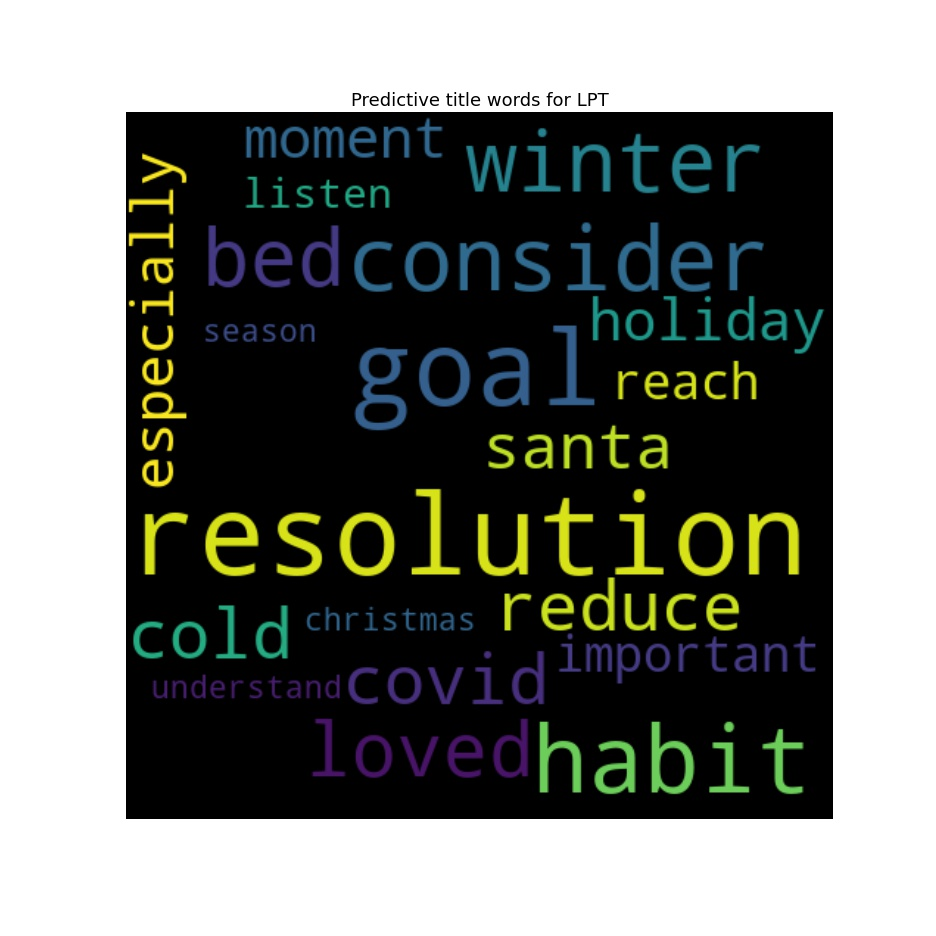
\includegraphics[width=12cm]{LPT_title_wordcloud.jpeg}
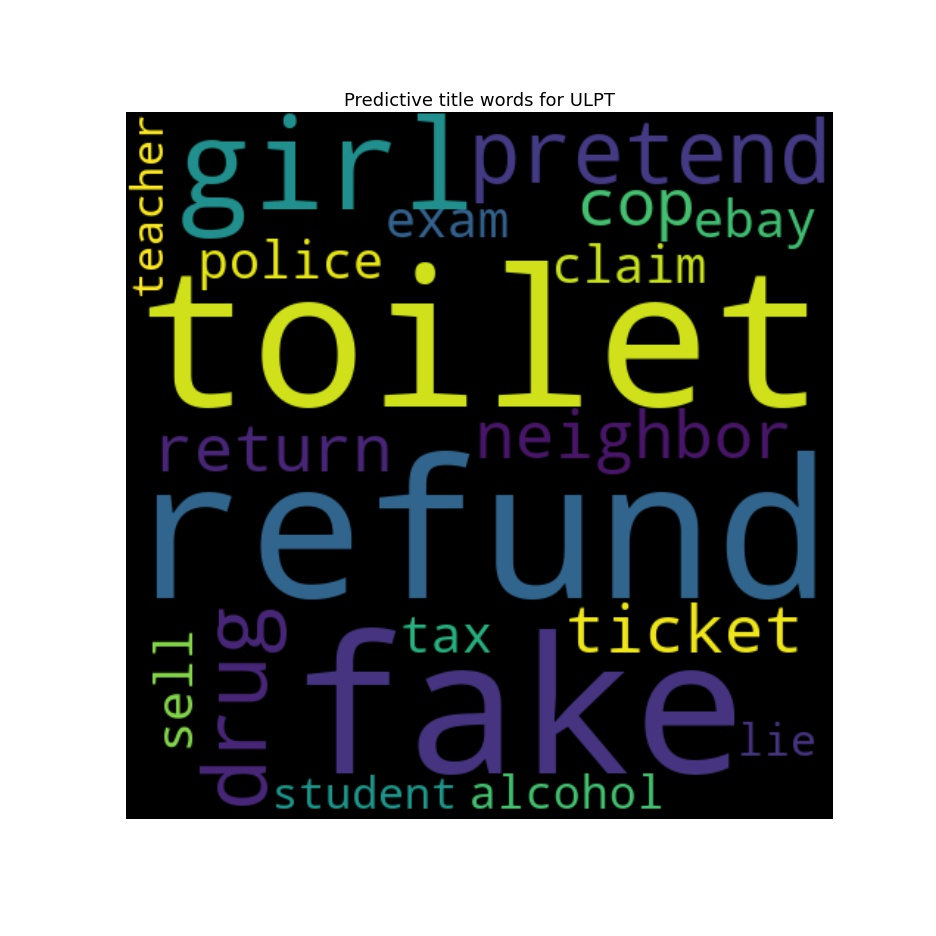
\includegraphics[width=12cm]{ULPT_title_wordcloud.jpeg}
\captionof{figure}{\small{Wordcloud for most predictive \texttt{title} words for each subreddit}}
\label{lpt_wordcloud} 
\end{figure}
%
%\subsubsection{LifeProTips most predictive words}
The top three words are \tql resolution,\tqr \tql goal,\tqr and \tql habit.\tqr. Each word in the wordcloud aligns (allowing for seasonal considerations) with the observation that posts from LifeProTips are of a self-improvement nature.



%\begin{enumerate}
%
%\item \textbf{\tql resolution\tqr} 
%%The conditional probability that a post comes from LifeProTips given that it contains the word \tql resolution\tqr is 0.98.  In fact, only one UnethicalLifeProTips post contains the word \tql resolution.\tqr Here are two examples from LifeProTips:
%
%\begin{itemize}
%
%\item \begin{quote}
%\tql New Year's Resolutions do not need to be about change.\tqr
%\end{quote}
%
%\item \begin{quote}
%\tql If you do not wash your teeth two times a day already, make it your new year's resolution to do it.\tqr
%\end{quote}
%
%\end{itemize}
%
%%\noin Here is the singular post from UnethicalLifeProTips:
%%
%%\begin{itemize}
%%
%%\item \begin{quote}
%%\tql If you are at an online meeting where you don't want to keep your camera on download a program like Altercam where you can edit your webcam settings and limit the FPS to 1 and resolution to the lowest so it looks so bad you can't see a thing or they ask you to turn it off.\tqr
%%\end{quote}
%%
%%\end{itemize}
%
%\item \textbf{\tql goal\tqr} 
%%The conditional probability that a post comes from LifeProTips given that it contains the word \tql goal\tqr is 0.95.  In fact, only three UnethicalLifeProTips posts contain the word \tql goal.\tqr  Two examples from LifeProTips:
%
%\begin{itemize}
%
%\item \begin{quote}
%\tql Whenever you set a goal (whether it’s a fitness, finance, or career goal), get an accountability partner. Having someone you trust check in on your progress can make the difference between hitting your goal or not\tqr
%\end{quote}
%
%\item \begin{quote}
%\tql If you made a goal to do X daily, remember that what you're really doing is creating a habit, and that can be difficult. Don't give up if you've missed a day or two early on, as the hardest part of creating a habit is the formation.\tqr
%\end{quote}
%
%\end{itemize}
%
%%\noin The author chooses not to share any of the UnethicalLifeProTips posts containing \tql goal.\tqr
%
%
%
%\item \textbf{\tql habit\tqr} 
%%The conditional probability that a post comes from LifeProTips given that it contains the word \tql habit\tqr is 0.92.  Only three UnethicalLifeProTips posts contain the word \tql habit.\tqr. Two examples from LifeProTips:
%
%\begin{itemize}
%
%\item \begin{quote}
%\tql If you want to stick to a new habit, try practicing it once a week instead of daily\tqr
%\end{quote}
%
%\item \begin{quote}
%\tql If you want to adopt a new habit, reframe the behavior change as a “standard,” instead of a “rule.” It’s easier to meet a standard than it is to try not to break a rule.\tqr
%\end{quote}
%
%\end{itemize}
%
%%\noin Here is an example of one of the rare posts from UnethicalLifeProTips containing the word \tql habit:\tqr
%%
%%\begin{itemize}
%%
%%\item \begin{quote}
%%\tql Get in the habit of playing Rock Paper Scissors with people, but make sure you consistently lose with the same throw. Eventually they will learn to expect the same throw and you can win any game you actually care about.\tqr
%%\end{quote}
%%
%%\end{itemize}
%
%
%\end{enumerate}
%
%\subsubsection{UnethicalLifeProTips most predictive words}

The top three predictive words for UnethicalLifeProTips are \tql refund,\tqr \tql toilet,\tqr and \tql fake.\tqr The presence of \tql refund\tqr and \tql fake\tqr and many others in the wordcloud is not surprising considering the theme of dishonesty underscoring most of the posts in the subreddit.  However, \tql toilet\tqr needs some more explanation: it turns out that there are many posts on how to get free toilet paper.  These align with the toilet paper shortage during the early days of the COVID-19 pandemic. For example:
\begin{itemize}

\item\begin{quote}
\tql Need toilet roll? Public bathrooms, free and fully stocked.\tqr
\end{quote}

\end{itemize}
Another word's appearance in the wordcloud is slightly puzzling at first: \tql girl.\tqr The word \tql girl\tqr turns out to be the fourth most predictive word for UnethicalLifeProTips.  From reviewing the data there are several different themes for this word on the UnethicalLifeProTips subreddit. One theme is posing as a girl on the internet:
\begin{itemize}

\item\begin{quote}
\tql Pretending to be a girl online to get free stuff\tqr
\end{quote}

\end{itemize}
Another major theme is \tql dating\tqr advice:
\begin{itemize}

\item\begin{quote}
\tql Save your side guy or girl’s number in your phone as Potential Spam. This way it will not cause alarm if your boyfriend/girlfriend sees them calling you.\tqr
\end{quote}

\item\begin{quote}
\tql See an pretty girl at the grocery but too shy to approach her? Go to the pet food aisle and put the biggest bag of dog food into your cart. Then push your cart down the aisle she’s on and boom, she’ll probably start talking to you first.\tqr
\end{quote}

\end{itemize}


%We will also take a close look at the top three most predictive words.
%
%\begin{figure}
%\centering
%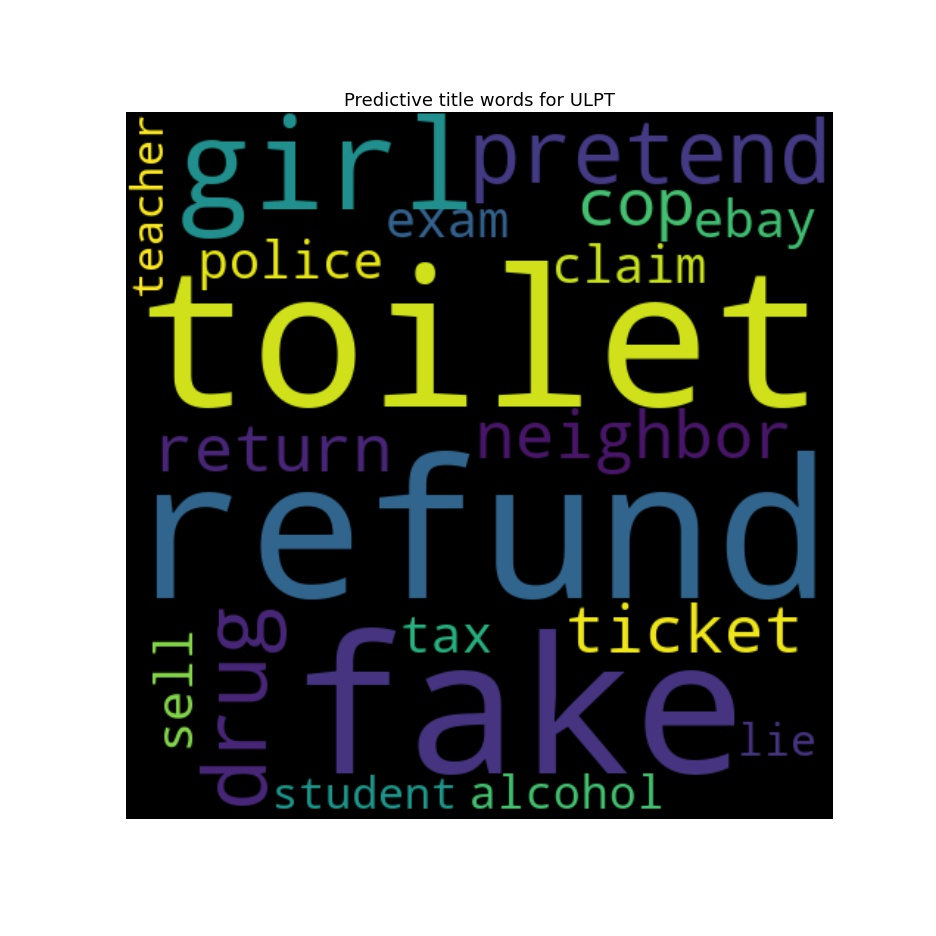
\includegraphics[width=10cm]{ULPT_title_wordcloud.jpeg}
%\captionof{figure}{\small{wordcloud for most predictive \texttt{title} words for UnethicalLifeProTips subreddit}}
%\label{ulpt_wordcloud} 
%\end{figure}
%
%\begin{enumerate}
%
%\item \textbf{\tql refund\tqr} The conditional probability that a post comes from UnethicalLifeProTips given that it contains the word \tql refund\tqr is 0.95.  Only seven LifeProTips posts contain the word \tql refund.\tqr Two examples from UnethicalLifeProTips:
%
%\begin{itemize}
%
%\item \begin{quote}
%\tql Order anything the last few months online? Complain it arrived damaged; they are so swamped most companies are automatically offering compensation/part refunds\tqr
%\end{quote}
%
%\item \begin{quote}
%\tql Need a power tool that you'll only use once? Buy it and refund it!\tqr
%\end{quote}
%
%\end{itemize}
%
%\noin Here is an example of a post from LifeProTips containing the word \tql refund:\tqr
%
%\begin{itemize}
%
%\item \begin{quote}
%\tql Never toss mail in the trash, before opening it, just because you think it is another bill/statement/etc.; it may actually be a refund!\tqr
%\end{quote}
%
%\end{itemize}
%
%\item \textbf{\tql toilet\tqr} The conditional probability that a post comes from UnethicalLifeProTips given that it contains the word \tql toilet\tqr is 0.94.  Only four LifeProTips posts contain the word \tql toilet.\tqr Two examples from UnethicalLifeProTips:
%
%\begin{itemize}
%
%\item \begin{quote}
%\tql Need toilet roll? Public bathrooms, free and fully stocked.\tqr
%\end{quote}
%
%\item \begin{quote}
%\tql Hate using shared restroom stalls at work? Wait until the janitor cleans the bathroom and then place an “out of order” sign on your favorite stall. You’ll enjoy a personal, clean toilet for a few weeks until the janitor and maintenance team coordinate.\tqr
%\end{quote}
%
%\end{itemize}
%
%\noin Here is an example of a post from LifeProTips containing the word \tql toilet:\tqr
%
%\begin{itemize}
%
%\item \begin{quote}
%\tql Clean your toilets now so if you have a rough New Year’s, at least you’ll have a clean throne\tqr
%\end{quote}
%
%\end{itemize}
%
%\item \textbf{\tql fake\tqr} The conditional probability that a post comes from UnethicalLifeProTips given that it contains the word \tql fake\tqr is 0.92.  Only eleven LifeProTips posts contain the word \tql fake.\tqr Two examples from UnethicalLifeProTips:
%
%\begin{itemize}
%
%\item \begin{quote}
%\tql have enough money for a rental but don’t meet the income requirement? Submit fake paystubs.\tqr
%\end{quote}
%
%\item \begin{quote}
%\tql If you need an Ambulance, leave your wallet behind and give fake identity information to the EMT. You'll never be billed for the ambulance ride.\tqr
%\end{quote}
%
%\end{itemize}
%
%\noin Here is an example of a post from LifeProTips containing the word \tql fake:\tqr
%
%\begin{itemize}
%
%\item \begin{quote}
%\tql if you think a login page is suspicious, don't enter your real password, enter something random - if it is fake it will proceed with the login\tqr
%\end{quote}
%
%\end{itemize}
%
%\end{enumerate}

\section{Modeling}\label{modeling}



\subsection{Model assessment}

We first apply the selected vectorizers to the \texttt{title} and \texttt{alltext} columns in the training data and concatenate using \texttt{scipy.sparse.hstack} together with the \texttt{title\_reading\_level} column (passed as a sparse matrix). We then perform 5-fold cross-validation with three different estimators: \texttt{RandomForestClassifier, MultinomialNB, LogisticRegression} in \texttt{sklearn}; for \texttt{MultinomialNB}, we ignore the \texttt{title\_reading\_level} column. We score the cross-validation with both the accuracy metric and the ROC-AUC metric.  Since the data is balanced, accuracy is a meaningful metric.  Table \ref{cv} provides the results from these cross-validations along with the performance on the test data.

\begin{table}
\caption{Cross-validation results}\label{cv}
\begin{tabular}{|p{0.3\linewidth}|p{0.3\linewidth}|p{0.2\linewidth}|p{0.1\linewidth}|}
\hline
Estimator & Hyperparameters & Mean CV Accuracy & Test Accuracy\\
\hline
\texttt{RandomForestClassifier} & \texttt{criterion='gini', max\_depth=78, max\_features='log2', n\_estimators=143} & 0.7614 & 0.7880\\
\hline
\texttt{MultinomialNB} & \texttt{alpha=1} & 0.7772 &0.7917 \\
\hline
\texttt{LogisticRegression} & \texttt{C=0.1, dual=False, penalty='l2', tol=0.0001} & 0.7714 & 0.8022\\
\hline
\end{tabular}
\end{table}


\subsection{Threshold tuning}
The next step is to tune the threshold for each estimator since each estimator in truth returns a probability value for its predictions.  We need to select the best threshold for each of our use-case.  We wish to use this model as an automated filter for unethical content.  Such a model would be used by social media moderators, internal business communications, online forums, etc.  The automated aspect of the model is intended to significantly reduce manual monitoring, so we choose to prioritize reducing false positives (a positive label belonging to the UnethicalLifeProTips subreddit).  This means we place more emphasis on obtaining a higher precision at the cost of a lower recall.  After examining the precision-recall curves for the three estimators above, we choose the \texttt{RandomForestClassifier} estimator with threshold 0.5718 to obtain a precision of 89.03\% with a recall of 50.20\%.  Figure \ref{RF_precision_recall} shows the precision recall curve for the \texttt{RandomForestClassifier} estimator, and Table \ref{RF_cm} shows the confusion matrix for this the selected threshold. This means that out of all of the posts predicted to be from the UnethicalLifeProTips subreddit, just under 9 out of 10 are truly from the ULPT subreddit, and out of all the posts that are truly from the ULPT subreddit, about 1 out of 2 are flagged by the model.  

\begin{figure}
\centering
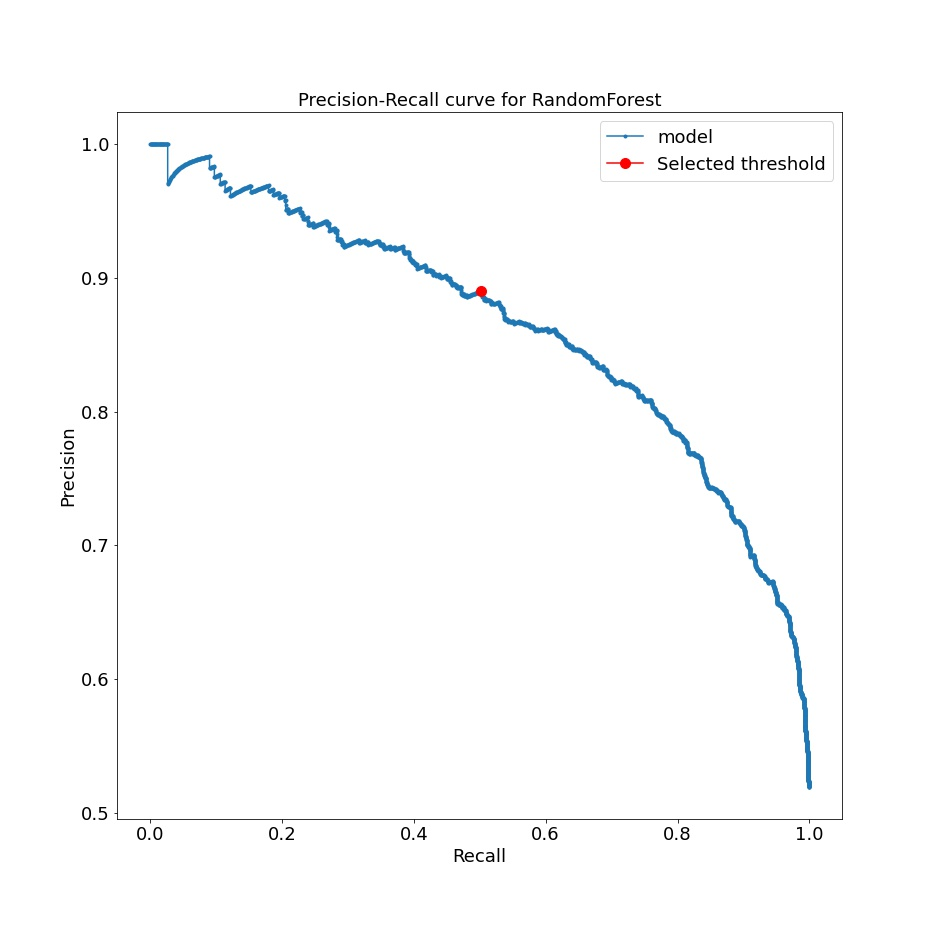
\includegraphics[width=12cm]{RF_precision_recall.jpeg}
\captionof{figure}{\small{Precision-recall curve for \texttt{RandomForestClassifier}, predicting membership of a post in the UnethicalLifeProTips subreddit.  The position of the selected threshold is indicated in red.}}
\label{RF_precision_recall} 
\end{figure}




\begin{table}
\caption{Confusion matrix for \texttt{RandomForestClassifier} with threshold 0.5718 predicting ULPT}\label{RF_cm}
\[\begin{array}{|c|c|c|}
\hline
& \text{Predicted False} & \text{Predicted True}\\
\hline
\text{Actual False} & 47.0\% & 3.2\%\\
\hline
\text{Actual True} & 24.6\% & 25.2\%\\
\hline
\end{array}\]
\end{table}







\section{Conclusion}\label{conclusion}

For most of the posts in this dataset, any individual with a reasonable amount of cultural and ethical awareness can accurately select which subreddit a given post comes from.  The data indicate that a piece of advice offering self-improvement that can be achieved by an individual alone is likely to come from LifeProTips, and a piece of advice suggesting dishonest behavior to gain something from others is likely to come from UnethicalLifeProTips. 
%But as we have seen, it takes more work to train a computer to make such distinctions. 

Overall LifeProTips reading levels are slightly higher than those of UnethicalLifeProTips. Thanks to our clustering via \texttt{LatentDirichletAllocation}, some common themes for these subreddits have been recognized:
\begin{itemize}

	\item \textbf{LifeProTips:} Resolutions, Cooking/kitchen, Money, Gift Giving, Mental health, Cleaning, Online behavior
	
	\item \textbf{UnethicalLifeProTips:} Avoid paywalls/ads, Scam return policies/rewards programs, Get out of work, Interpersonal spite/prank, Get something for nothing, Car related

\end{itemize}
The top three predictive words for each subreddit are as follows:
\begin{itemize}
	
	\item \textbf{LifeProTips:}
	
		\begin{enumerate}
		
			\item \tql resolution\tqr
			
			\item \tql goal\tqr
			
			\item \tql habit\tqr
		
		\end{enumerate}
	
	\item \textbf{UnethicalLifeProTips:}
	
		\begin{enumerate}
		
			\item \tql refund\tqr
			
			\item \tql toilet\tqr
			
			\item \tql fake\tqr
		
		\end{enumerate}
	
\end{itemize}

We obtained a binary classification model with precision 89.03\% and recall 50.20\% predicting a post's membership in the UnethicalLifeProTips subreddit.  Such high precision indicates that the model is effective in that when it identifies a post as unethical, it is correct 9 out of 10 times.  This greatly reduces the need for manual monitoring for forum moderation.  The recall, much lower than the precision, shows that 1 out of every 2 unethical posts goes undetected.

It is worth noting that the content from the subreddits is in the form of advice.  So this model is trained to specifically recognize unethical advice rather than more general unethical content.  Furthermore, the motivation for writing each post seems to differ across the subreddits: LifeProTips are more sincere, UnethicalLifeProTips are a mix of sincerity, spite, and humor.

This model can be strengthened and made more accurate with more data.  We could scrape many more posts from the two subreddits to provide more training data and make the model more robust.  We could also set up a remote server to periodically scrape more data from the subreddits and automatically retrain the model.

%\subsection*{Acknowledgment} The author would like to thank his Springboard mentor Ben Bell for his helpful guidance throughout this project.




\end{document}